\documentclass[reqno]{amsart}
\usepackage{amscd, amssymb, amsmath, amsthm}
\usepackage{graphicx}
\usepackage[colorlinks=true,linkcolor=blue]{hyperref}
\usepackage[utf8]{inputenc}
\usepackage[T1]{fontenc}
\usepackage{textcomp}
\usepackage{babel}
%% for identity function 1:
\usepackage{bbm}
%%For category theory diagrams:
\usepackage{tikz-cd}

%\usepackage[backend=biber]{biblatex}
%\addbibresource{.bib}


\setlength\parindent{0pt}

\pdfsuppresswarningpagegroup=1

\newtheorem{theorem}{Theorem}[section]
\newtheorem{lemma}[theorem]{Lemma}
\newtheorem{proposition}[theorem]{Proposition}
\newtheorem{corollary}[theorem]{Corollary}
\newtheorem{conjecture}[theorem]{Conjecture}

\theoremstyle{definition}
\newtheorem{definition}[theorem]{Definition}
\newtheorem{example}[theorem]{Example}
\newtheorem{exercise}[theorem]{Exercise}
\newtheorem{problem}[theorem]{Problem}
\newtheorem{question}[theorem]{Question}

\theoremstyle{remark}
\newtheorem*{remark}{Remark}
\newtheorem*{note}{Note}
\newtheorem*{solution}{Solution}



%Inequalities
\newcommand{\cycsum}{\sum_{\mathrm{cyc}}}
\newcommand{\symsum}{\sum_{\mathrm{sym}}}
\newcommand{\cycprod}{\prod_{\mathrm{cyc}}}
\newcommand{\symprod}{\prod_{\mathrm{sym}}}

%Linear Algebra

\DeclareMathOperator{\Span}{span}
\DeclareMathOperator{\im}{im}
\DeclareMathOperator{\diag}{diag}
\DeclareMathOperator{\Ker}{Ker}
\DeclareMathOperator{\ob}{ob}
\DeclareMathOperator{\Hom}{Hom}
\DeclareMathOperator{\Mor}{Mor}
\DeclareMathOperator{\sk}{sk}
\DeclareMathOperator{\Vect}{Vect}
\DeclareMathOperator{\Set}{Set}
\DeclareMathOperator{\Group}{Group}
\DeclareMathOperator{\Ring}{Ring}
\DeclareMathOperator{\Ab}{Ab}
\DeclareMathOperator{\Top}{Top}
\DeclareMathOperator{\hTop}{hTop}
\DeclareMathOperator{\Htpy}{Htpy}
\DeclareMathOperator{\Cat}{Cat}
\DeclareMathOperator{\CAT}{CAT}
\DeclareMathOperator{\Cone}{Cone}
\DeclareMathOperator{\dom}{dom}
\DeclareMathOperator{\cod}{cod}
\DeclareMathOperator{\Aut}{Aut}
\DeclareMathOperator{\Mat}{Mat}
\DeclareMathOperator{\Fin}{Fin}
\DeclareMathOperator{\rel}{rel}
\DeclareMathOperator{\Int}{Int}
\DeclareMathOperator{\sgn}{sgn}
\DeclareMathOperator{\Homeo}{Homeo}
\DeclareMathOperator{\SHomeo}{SHomeo}
\DeclareMathOperator{\PSL}{PSL}
\DeclareMathOperator{\Bil}{Bil}
\DeclareMathOperator{\Sym}{Sym}
\DeclareMathOperator{\Skew}{Skew}
\DeclareMathOperator{\Alt}{Alt}
\DeclareMathOperator{\Quad}{Quad}
\DeclareMathOperator{\Sin}{Sin}
\DeclareMathOperator{\Supp}{Supp}
\DeclareMathOperator{\Char}{char}
\DeclareMathOperator{\Teich}{Teich}
\DeclareMathOperator{\GL}{GL}
\DeclareMathOperator{\tr}{tr}
\DeclareMathOperator{\codim}{codim}
\DeclareMathOperator{\coker}{coker}
\DeclareMathOperator{\corank}{corank}
\DeclareMathOperator{\rank}{rank}
\DeclareMathOperator{\Diff}{Diff}
\DeclareMathOperator{\Bun}{Bun}
\DeclareMathOperator{\Sm}{Sm}
\DeclareMathOperator{\Fr}{Fr}
\DeclareMathOperator{\Cob}{Cob}
\DeclareMathOperator{\Ext}{Ext}
\DeclareMathOperator{\Tor}{Tor}
\DeclareMathOperator{\Conf}{Conf}
\DeclareMathOperator{\UConf}{UConf}



%Row operations
\newcommand{\elem}[1]{% elementary operations
\xrightarrow{\substack{#1}}%
}

\newcommand{\lelem}[1]{% elementary operations (left alignment)
\xrightarrow{\begin{subarray}{l}#1\end{subarray}}%
}

%SS
\DeclareMathOperator{\supp}{supp}
\DeclareMathOperator{\Var}{Var}

%NT
\DeclareMathOperator{\ord}{ord}

%Alg
\DeclareMathOperator{\Rad}{Rad}
\DeclareMathOperator{\Jac}{Jac}

%Misc
\newcommand{\SL}{{\mathrm{SL}}}
\newcommand{\mobgp}{{\mathrm{PSL}_2(\mathbb{C})}}
\newcommand{\id}{{\mathrm{id}}}
\newcommand{\MCG}{{\mathrm{MCG}}}
\newcommand{\PMCG}{{\mathrm{PMCG}}}
\newcommand{\SMCG}{{\mathrm{SMCG}}}
\newcommand{\ud}{{\mathrm{d}}}
\newcommand{\Vol}{{\mathrm{Vol}}}
\newcommand{\Area}{{\mathrm{Area}}}
\newcommand{\diam}{{\mathrm{diam}}}
\newcommand{\End}{{\mathrm{End}}}


\newcommand{\reg}{{\mathtt{reg}}}
\newcommand{\geo}{{\mathtt{geo}}}

\newcommand{\tori}{{\mathcal{T}}}
\newcommand{\cpn}{{\mathtt{c}}}
\newcommand{\pat}{{\mathtt{p}}}

\let\Cap\undefined
\newcommand{\Cap}{{\mathcal{C}}ap}
\newcommand{\Push}{{\mathcal{P}}ush}
\newcommand{\Forget}{{\mathcal{F}}orget}




\begin{document}

\section{Cohomology and Homological Algebra}

\subsection{Cohomology in terms of Homological Algebra}

    Recall the Universal Coefficient Theorem for Cohomology:

    \begin{theorem}[Universal Coefficient Theorme for Cohomology]
        Let $R$ be a ring and $A$ an $R-$ module. Let
        $C_*$ be a complex of projective $R$-modules
        such that the subcomplex of boundaries 
        $B_*$ is also a complex of projective modules.
        \begin{enumerate}
            \item For all $n$, there is a SES
                \[
                0 \to \Ext_R^{1} \left( 
                H_{n-1}(C_*),A\right) \stackrel{\lambda_n}{\to} 
                H^{n} \left( \Hom_R \left( C_*,A \right)  \right) 
                \stackrel{\mu_n}{\to} \Hom_R \left( 
                H_n \left( C_* \right), A \right) \to 0
                \] 
                where both $\lambda_n$ and $\mu_n$ are
                natural in $C_*$ and $A$.
            \item If $R$ is a PID, then the SES in (1) is
                split, but it is not always naturally split.
        \end{enumerate}
    \end{theorem}

    Also recall the basic properties:

    \begin{lemma}[]
        For a finitely generated $H$, we have
        \begin{itemize}
            \item $\Ext \left( 
                H \oplus H' , G\right) \cong
                \Ext \left( H, G \right) \oplus
                \Ext(H',G)$
            \item $\Ext (H,G) = 0$ if $H$ is free.
            \item $\Ext (\mathbb{Z} / n, G) \cong
                G / n G$.
        \end{itemize}
    \end{lemma}

    \begin{corollary}\label{Cor:JSIOA}
        If the homology groups $H_n$ and
        $H_{n-1}$ of a chain complex
        $C$ of free abelian groups are finitely
        generated, with torsion subgroups
        $T_n \subset H_n$ and 
        $T_{n-1} \subset H_{n-1}$, then
        $H^{n}( \Hom_\mathbb{Z} (C_*, \mathbb{Z}) ) \cong
        \left( H_n / T_n \right) \oplus T_{n-1}$.
    \end{corollary}

    \begin{proof}
        By the Universal Coefficient theorem for cohomology, we
        have that
        \[
        H^{n} \left( 
        \Hom_\mathbb{Z} \left( C_*, \mathbb{Z} \right) \right) 
        \cong
        \Ext_{\mathbb{Z}}^{1} 
        \left( H_{n-1}(C_*), \mathbb{Z} \right) 
        \oplus \Hom_{\mathbb{Z}} \left( 
        H_n \left( C_*\right), \mathbb{Z} \right) 
        \] 
        Now,
        $\Ext_{\mathbb{Z}}^{1} \left( H_{n-1}(C_*),\mathbb{Z}
        \right) \cong T_{n-1}$ and
        $\Hom_{\mathbb{Z}} \left( H_n
        \left( C_* \right), \mathbb{Z} \right) 
        \cong H_n / T_n$.
    \end{proof}

    \begin{proposition}[]
        If a chain map between chain complexes of free
        abelian groups induces an isomorphism on homology
        groups, then it induces an isomorphism
        on cohomology groups with any coefficient
        group $G$.
    \end{proposition}

    \begin{proof}
        Suppose
        $\alpha \colon C_* \to C_*'$ is the chain map
        such that $\alpha_* \colon
        H_n (C_*) \to H_n (C_*')$ is an isomorphism
        for all $n$.
        Consider the diagram

        \begin{equation*}
        \begin{tikzcd}
            0 \ar[r] & 
            \Ext \left( H_{n-1}(C),G \right) 
            \ar[r] & H^{n}(C;G) \ar[r, "h"] &
            \Hom(H_n(C),G) \ar[r] & 0\\
            0 \ar[r] & 
            \Ext(H_{n-1}(C'),G) \ar[r] \ar[u, "(\alpha_*)^{*}",
            "\cong"']
                     & H^{n}(C';G) \ar[r, "h"] \ar[u, "\alpha^*"] 
                     & \Hom(H_n (C'),G) \ar[r] 
            \ar[u, "(\alpha_*)^{*}", "\cong"'] & 0
        \end{tikzcd}
        \end{equation*}
        which follows form naturality of the
        Universal Coefficient theorem.
        Then by the $5$-lemma, we obtain that
        $\alpha^*$ is an isomorphism also.
        
    \end{proof}



    \subsection{Cohomology of Spaces}


    Define
    $S^{-n} (X;A) :=
    \Hom_{\mathbb{Z}} \left( S_n(X),A \right) $,
    so $S^{*}(X;A)$ is a chain complex.
    We define
    $H^{n}(X;A) :=
    H_{-n}\left( S^{*}(X;A) \right) $, called \textit{singular
    cohomology of $X$ with coefficients in $A$.}\\

    Thus an $n$-cochain $\varphi 
    \in S^{-n}(X;G)$ assigns to each
    $n$-simplex $\sigma \colon \Delta^{n} \to X$ a
    value $\varphi \left( \sigma \right) \in G$.
    Since the $n$-simplicies form a basis for
    $S_n(X)$, these values can be chosen arbitrarily,
    hence $n$-cochains are exactly equivalent to functions
    from singular $n$-simplices to $G$.\\
    The \textit{coboundary map} $\delta
    \colon S^{-n}(X;G) \to S^{-(n+1)}(X;G)$ is the dual
     $\partial^{*}$, so for
     a cochain $\varphi \in 
     S^{-n}(X;G)$, its coboundary $\delta
     \varphi  $ is the composition
     $\delta \varphi  = 
     \partial^{*} \varphi =
     \varphi \circ \partial$, i.e., the composition
     $C_{n+1} (X) \stackrel{\partial}{\to} 
     C_n(X) \stackrel{\varphi }{\to} G$.

     Hence for a singular $(n+1)$-simplex
     $\sigma \colon \Delta^{n+1} \to X$, we have
     \[
     \delta \varphi (\sigma) = 
     \sum_{i} (-1)^{i} 
     \varphi \left( \sigma |_{\left[ v_0, \ldots,
     \widehat{v_i}, \ldots, v_{n+1}\right] } \right).
     \] 
     Since $\delta^2$ is the dual of
     $\partial^2 = 0$, we have
     $\delta^2 = 0$ also, so
     $H^{n}(X;G)$ can be defined as above.\\
     \linebreak
     \begin{note}
         For a cochain $\varphi \in 
         S^{-n}(X;G)$ to be a cocyle means that
         $\delta \varphi = \varphi \partial = 0$, i.e.,
         it means that $\varphi $ vanishes on boundaries.
     \end{note}

     \subsubsection{$H^{0}$ :} When $n = 0$, there
     is no $\Ext$ term and so
     $H^{0}(X;G) \cong \Hom (H_0(X),G)$.
     This can also be sen from definitions: singular
     $0$-simplices are just points of $X$, so
     a cochain in $S^{0}(X;G)$ is an
     arbitrary function $\varphi  \colon
     X \to G$, not necessarily continuous. For this to
     be a cocycle, we must have
     $0 = \delta \varphi = 
     \varphi \circ \partial $. Evaluating this
     at some $1$-simplex $\left[ v_0, v_1 \right] $, we
     find that $\varphi (v_1) - \varphi (v_0) = 0$, so
     $\varphi $ is simply constant on each path component.
     Thus $H^{0}(X;G)$ is just the set of all
     functions from the path components of $X$ into $G$, which 
     is the same as the set of all
     group homomorphisms from
     $S_0 (X)$ into $G$, i.e.,
     $H^{0}(X;G) \cong \Hom\left( H_0(X),G \right) $.

     \subsubsection{$H^{1}$ :} Likewise,
     $\Ext \left( H_0(X),G \right) = 0$ since
     $H_0(X)$ is free, so by the Universal Coefficient theorem,
     $H^{1}(X;G)$ is isomorphic to
     $\Hom\left( H_1(X),G \right)$ which, when
     $X$ is path-connected, is isomorphic to
     $\Hom\left( \pi_1(X),G \right) $ since $G$ is
     abelian.


     \subsubsection{Reduced Cohomology Groups}

     Reduced cohomology groups
     $\tilde{H}^{n}(X;G)$ can be defined by
     dualizing the augmented chain complex
     $\ldots \to C_0(X) \stackrel{\varepsilon}{\to} \mathbb{Z}
     \to 0$, then taking $\ker / \im$.
     This gives $\tilde{H}^{n}(X;G) = 
     H^{n}(X;G)$ for $n>0$, and the Universal Coefficient theorem
     gives $\tilde{H}^{0}(X;G) = 
     \Hom \left( \tilde{H}_0 (X),G \right) $.

     We can also describe 
     $\tilde{H}^{0}(X;G) \cong \Hom\left( \tilde{H}_0
     (X),G\right) $ more explicitly by using the above
     interpretation of $H^{0}(X;G)$ as functions
     $X \to G$ which are constant on path-components.
     Recall that $\varepsilon \colon
     C_0(X) \to \mathbb{Z}$ sends each
     singular $0$-simplex $\sigma$ to $1$, so
     $\varepsilon^{*}$ sends
     a homomorphism
     $\varphi  \colon \mathbb{Z} \to G$ to
     $C_0(X) \stackrel{\varepsilon}{\to} \mathbb{Z}
     \stackrel{\varphi }{\to} G$ which sends
     $\sigma \mapsto \varphi (1)$ for all
     $0$-simplices. That is,
     $\varepsilon^{*}\varphi $ is a constant
     function $X \to G$, and since
     $\varphi (1)$ can be any element of
     $G$, the image of $\varepsilon^{*}$ consists of precisely
     the constant functions.
     Thus $\tilde{H}^{0}(X;G)$ is all
     functions $X \to G$ that are constant on path-components
     modulo the functions that are constant on all of $X$.


     \subsubsection{Relative Groups and the LES of a Pair}

     To define relative groups
     $H^{n}(X,A;G)$ for a pair $(X,A)$, we first
     dualize the SES
     \[
     0 \to S_n(A) \stackrel{i}{\to} 
     S_n(X) \stackrel{j}{\to} 
     S_n(X,A) \to 0
     \] 
     by applying $\Hom(-,G)$ to get
     \[
     0 \leftarrow S^{n}(A;G) 
     \stackrel{i^{*}}{\leftarrow}
     S^{n}(X;G) \stackrel{j^{*}}{\leftarrow}
     S^{n}(X,A;G) \leftarrow 0 \tag{$\Omega$}\label{Omega}
     \] 
     where 
     $S^{n}(X,A;G) := \Hom \left( C_n (X,A),G \right) $.

     To see exactness of the dual sequence,
     we note the following:
     $i^{*}$ restricts cochains on $X$ to cochains
     on $A$, so for a function
     from singular $n$-simplices in $X$ to $G$, the
     image of this function under
     $i^{*}$ is obtained by restricting the domain of the
     function to singular $n$-simplices in $A$.
     Every function from singular $n$-simplices in $A$
     to $G$ can be extended to all singular $n$-simplices
     in  $X$, for example, by assigning the value
     $0$ to all singular $n$-simplices not in  $A$, so
     $i^{*}$ is surjective. The kernel consists
     of cochains taking the value $0$ on all
     singular $n$-simplices in $A$.
     Such cochains are the same as
     homomorphisms $C_n (X,A) =
     C_n (X) / C_n(A) \to G$, so the kernel
     of $i^{*}$ is exactly $C^{n}(X,A;G) = 
     \Hom\left( C_n(X,A),G \right) $, giving the desired
     exactness.

     \begin{note}
         Note that we can view $C^{n}(X,A;G)$ as the
         functions from signular $n$-simplices in
         $X$ to $G$ that vanish on simplices
         in $A$, since the basis for $C_n(X)$ consisting
         of singular $n$-simplices in $X$ 
         is the disjoint union of the simplices
         with image contained in $A$ and the simplices
         with image no contained in $A$.
     \end{note}

     Relative coboundary maps
     $\delta \colon C^{n}(X,A;G) \to 
     C^{n+1}(X,A;G)$ are obtained as restrictions
     of the absolute $\delta$'s.\\
     \linebreak
     Since the maps
     $i^{*}$ and $j^{*}$ commute with
     $\delta$ (since $i$ and $j$ commute with $\partial$ ),
     the maps $i^{*}$ and $j^{*}$ induce
     chain maps
     $i^{*} \colon S^{*}(X;G) \to S^{*}(A;G)$ and
     $j^{*} \colon S^{*}(X,A;G) \to 
     S^{*}(X;G)$, and in particular, since
     $i^{*} j^{*} = 0$, this is a SES of
     chain complexes, hence induces a LES
     of cohomology groups (Thm. 6.5.5, AlgTop1):

     \[
     \ldots \to 
     H_n \left( S^{*}(X,A;G) \right) 
     \stackrel{j^{*}}{\to} 
     H_n \left( S^{*}(X;G) \right) 
     \stackrel{i^{*}}{\to} 
     H_n (S^{*}(A;G)) 
     \stackrel{\delta}{\to} 
     H^{n+1}(X,A;G) \to \ldots
     \] 
     By similar reasoning, one obtains a
     LES of reduced cohomology groups for a pair
     $(X,A)$ with $A$ nonempty.
     In particular, if $A$ is a point, we find
     $\tilde{H}^{n}(X;G) \cong
     H^{n}(X,x_0;G)$.\\
     \linebreak
     More generally, there is a LES for a triple
     $\left( X,A,B \right) $ coming from the
     SES
     \[
     0 \leftarrow C^{n}(A,B;G)
     \stackrel{i^{*}}{\leftarrow}
     C^{n}(X,B;G) \stackrel{j^{*}}{\leftarrow}
     C^{n}(X,A;G) \leftarrow 0.
     \] 


     \subsubsection{Duality between Connecting
     Homomorphisms}

     There is a duality between
     $\delta \colon
     H^{n}(A;G) \to H^{n+1}(X,A;G)$ and
     $\partial \colon
     H_{n+1}(X,A) \to H_n(A)$ as depicted in the
     following diagram:

     \begin{equation*}
     \begin{tikzcd}
         H^{n}(A;G) \ar[r, "\delta"] \ar[d,"h"] & 
         H^{n+1}(X,A;G) \ar[d, "h"] \\
         \Hom\left( H_n(A),G \right) 
         \ar[r, "\partial^{*}"] &
         \Hom \left( H_{n+1}(X,A),G \right) 
     \end{tikzcd}
     \end{equation*}
     
     \begin{proof}
         Recall that the connecting homomorphisms
         were defined by the diagrams
         \begin{equation*}
         \begin{tikzcd}
             & S^{n+1}(X;G) & S^{n+1}(X,A;G) \ar[l] \\
             S^{n}(A;G) \ar[rru, dashed] & S^{n}(X;G) \ar[u] 
             \ar[l]
         \end{tikzcd}
         \end{equation*}
         and

         \begin{equation*}
         \begin{tikzcd}
             & S_{n+1}(X) \ar[r] & S_{n+1}(X,A) \ar[dll, dashed]\\
             S_n(A) \ar[r] & S^{n}(X;G) \ar[u] &
         \end{tikzcd}
         \end{equation*}
         where the dashed arrows are
         only there when the chain and cochain groups
         are replaced by homology and cohomology groups.\\
         To see that $h \delta = \partial^{*} h$,
         let $\alpha \in H^{n}(A;G)$ be represented
         by a cocycle $\varphi  \in S^{n}(A;G)$.
         To compute $\delta (\alpha)$, first
         extend $\varphi $ to
         $\overline{\varphi }\in 
         S^{n}(X;G)$ by letting $\overline{\varphi }$ 
         be $0$ on all cochains not contained in
         $A$. Then
         composing $\overline{\varphi }$ with
         $\partial \colon S_{n+1}(X) \to S_n(X)$
         to get a cochain
         $\delta \overline{\varphi }
         = \overline{\varphi } \partial \in 
         S^{n+1}(X;G)$, and since
         $\varphi \in S^{n}(A;G)$ was a cocycle, we have
         that $\delta \varphi  = 0$, so
         $\overline{\varphi } \circ \partial$ is actually
         in $S^{n+1}(X,A;G)$ and represents
         $\delta \left( \alpha \right) \in 
         H^{n+1}(X,A;G)$.
         Now applying $h$ to $\overline{\varphi }
         \partial$ simply restricts the domain
         of $\overline{\varphi }\partial $ to relative
         cycles in $S_{n+1}(X,A)$, i.e., 
         $(n+1)$-chains in $X$ whose boundary lies in 
         $A$. On such chains
         $\overline{\varphi } \partial = 
         \varphi \partial$ since the extension of $\varphi $ 
         to $\overline{\varphi }$ has no effect here.
         Thus
         $h \delta \left( \alpha \right) $ is
         represented by $\varphi \partial$.\\
         One the other hand,
         let us consider $\partial^{*} h (\alpha)$.
         Recall that
         $S^{n}(X;A) = 
         \Hom_{\mathbb{Z}}\left( 
         S_n(X), A\right) $, so
         $\varphi $ is a homomorphism
         $S_n(X) \to A$. Applying $h$ to $\varphi $ then
         restricts the domain to  $n$-cycles in
         $A$. Then applying
         $\partial^{*}$ composes with the map
         which sends a relative $(n+1)$-cycle in
         $X$ to its boundary in $A$. Thus
         $\partial^{*} h \left( \alpha \right) $ 
         is represented by
         $\varphi \partial $ just as
         $h \delta (\alpha)$ was, hence the square commutes.

     \end{proof}


     \subsubsection{Induced Homomorphisms}

     If we have a chain map
     $f_{\#} \colon S_{*}(X) \to S_{*}(Y)$ induced
     by $f \colon X \to Y$, the we also have
     dual cochain maps
     $f^{\#}\colon S^{*}(Y;G) \to S^{n}(X;G)$.
     The relation
     $f_{\#} \partial = \partial f_{\#}$ dualizes
     to $\delta f^{\#} = f^{\#} \delta $, so
     $f^{\#}$ is a cochain chain map and hence
     induced homomorphisms
     $f^{*} \colon H^{n}(Y;G) \to H^{n}(X;G)$.\\
     In the relative case, a map
     $f \colon (X,A) \to (Y,B)$ induces
     $f^{*} \colon
     H^{n}(Y,B;G) \to H^{n}(X,A;G)$ by the same reasoning.

     Since $f$ induces a map between short exact
     sequences of cochain complexes, it induces a map between
     long exact sequences of cohomology groups
     with commuting squares.

     The properties
     $(fg)^{\#} = g^{\#} f^{\#}$ and
     $\id^{\#} = \id$ imply
     $\left( fg \right)^{*} = g^{*} f^{*}$ and
     $\id^{*} = \id$, so
     $X \mapsto H^{n}(X;G)$ and
     $(X,A) \mapsto H^{n}(X,A;G)$ are contravariant functors.\\
     \linebreak
     The algebraic Universal Coefficient theorem applies
     also to the relative cohomology since
     the relative groups $C_n (X,A)$ are free, and
     there is a naturality statement also:
     a map $f \colon (X,A) \to (Y,B)$ induces a commutative
     diagram

     \begin{equation*}
     \begin{tikzcd}
         0 \ar[r] & \Ext \left( H_{n-1}(X,A),G \right) 
         \ar[r] & H^{n}(X,A;G) \ar[r, "h"] &
         \Hom \left( H_n(X,A),G \right) \ar[r] & 0\\
         0 \ar[r] & \Ext \left( H_{n-1}(Y,B),G \right) 
         \ar[r] \ar[u, "(f_*)^{*}"] & 
         H^{n}(Y,B;G) \ar[r, "h"] \ar[u, "f^{*}"] &
         \Hom \left( H_n (Y,B),G \right) \ar[r]
         \ar[u, "(f_*)^{*}"] & 0
     \end{tikzcd}
     \end{equation*}


     \subsubsection{Axioms for Cohomology}

     These are exactly dual to the axioms for homology.
     Restricting attention to CW complexes, a
     (reduced) \textit{cohomology theory} is a sequence
     of contravariant functors
     $\tilde{h}^{n}$ from CW complexes to abelian
     groups, together with natural coboundary homomorphisms
     $\delta \colon \tilde{h}^{n}(A) \to 
     \tilde{h}^{n+1}(X /A)$ for CW pairs $(X,A)$, satisfying
     the following axioms:
     \begin{enumerate}
         \item If $f \simeq g \colon
             X \to Y$, then $f^{*} = g^{*}
             \colon \tilde{h}^{n}(Y) \to 
             \tilde{h}^{n}(X)$.
         \item For each CW pair $(X,A)$, there is a LES
             \[
             \ldots \stackrel{\delta}{\to} 
             \tilde{h}^{n}(X /A) \stackrel{q^{*}}{\to} 
             \tilde{h}^{n}(X) \stackrel{i^{*}}{\to} 
             \tilde{h}^{n}(A)
             \stackrel{\delta}{\to} 
             \tilde{h}^{n+1}(X /A) \stackrel{q^{*}}{\to} 
             \ldots
             \] 
         \item For a wedge sum $X = \bigvee_{\alpha} X_{\alpha}$ 
             with inclusions $i_{\alpha} \colon
             X_{\alpha} \hookrightarrow X$, the product
             map $\prod_{\alpha} i_{\alpha}^{*}
             \colon \tilde{h}^{n}(X) \to 
             \prod_{\alpha} \tilde{h}^{n}(X_{\alpha})$ is
             an isomorphism for each $n$.
     \end{enumerate}
     

     \subsubsection{Simplicial Cohomology}
     If $X$ is a $\Delta$-complex and
     $A \subset X$ is a subcomplex, then the
     simplciail chain groups $\Delta_n (X,A)$ dualize
     to simplicial cochain groups
     $\Delta^{n}(X,A;G) :=
     \Hom \left( \Delta_n (X,A),G \right) $, and the
     resulting cohomology groups are
     by definition the simplicial cohomology groups
     $H_{\Delta}^{n}(X,A;G)$. Since the inclusions
     $\Delta_n (X,A) \hookrightarrow C_n(X,A)$ induce
     isomorphisms 
     $H_n^{\Delta} \cong H_n (X,A)$, then
     Corollary \ref{Cor:JSIOA} implies that the
     dual maps
     $S^{n}(X,A;G) \to \Delta^{n}(X,A;G)$ also
     induce isomorphisms
     $H^{n}(X,A;G) \cong
     H_{\Delta}^{n}(X,A;G)$.




     \begin{exercise}[]
         \begin{enumerate}
             \item Directly from the definitions, compute
                 the simplicial cohomology
                 groups of $S^{1} \times S^{1}$ with
                 $\mathbb{Z}$ and $\mathbb{Z}_2$ coefficients,
                 using the product $\Delta$-complex structure.
             \item Do the same for $\mathbb{R}\mathbb{P}^2$ and
                 the Klein bottle.
         \end{enumerate}
     \end{exercise}

     \begin{solution}
         We are asked to do it directly from definitions, so
         let us track through each step:
         we can give $S^{1} \times S^{1} =: T$ the
         $\Delta$-complex structure indicated Figure
         \ref{fig:Figures-Delta-for-T-png}.
         
         \begin{figure}[htpb]
             \centering
             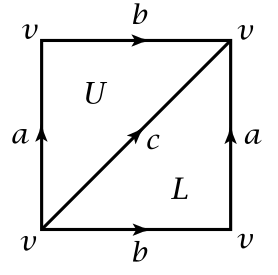
\includegraphics[width=0.25\textwidth]{Figures/Delta-for-T.png}
             \caption{}
             \label{fig:Figures-Delta-for-T-png}
         \end{figure}

         Then
         $\Delta_n (S^{1} \times S^{1})
         \cong
         \begin{cases}
             \mathbb{Z}^2,& n=2\\
             \mathbb{Z}^3,& n=1\\
             \mathbb{Z},& n=0\\
             0,& \text{else}
         \end{cases}$ 
         And in particular, we get a chain complex
         \[
         0 \to \mathbb{Z}^2 
         \stackrel{
         \begin{pmatrix} 
             1 & -1\\
             -1 & 1\\
             1 & 1
     \end{pmatrix} }{\to}   \mathbb{Z}^3 
     \stackrel{0}{\to} \mathbb{Z} \to 0
         \] 
         so dualizing, we get
         that since  $\Hom(\mathbb{Z}^{k},\mathbb{Z})
         \cong \mathbb{Z}^{k}$, then the dual complex
         becomes

         \[
         0 \leftarrow \mathbb{Z}^2 
         \stackrel{
         \begin{pmatrix} 
             1 & -1\\
             -1 & 1\\
             1 & 1
     \end{pmatrix}^{*} }{\leftarrow}   \mathbb{Z}^3 
     \stackrel{0}{\leftarrow} \mathbb{Z} \leftarrow 0.
         \] 
         By linear algebra, we know that
         the dual of a matrix is given by its transpose, so
         this chain complex becomes

         \[
         0 \leftarrow \mathbb{Z}^2 
         \stackrel{
         \begin{pmatrix} 
             1 & -1 & 1\\
             -1 & 1 & 1
     \end{pmatrix}}{\leftarrow}   \mathbb{Z}^3 
     \stackrel{0}{\leftarrow} \mathbb{Z} \leftarrow 0.
         \] 
         From this, we can read off the homology groups
         of the chain complex.
         In degree $2$, $\ker \delta = \mathbb{Z}^2$, so
         \[
         H^{2}(S^{1} \times S^{1}; \mathbb{Z})
         \cong
         \mathbb{Z}^2 / \left( U = L,
         U = -L \right) \cong
         0.
         \] 
         For $H^{1}$, the kernel
         of the transposed matrix
         is
         $\ker \delta  =
         \left< 
         \begin{pmatrix} 1 \\ 1 \\ 0 \end{pmatrix} \right>$ which
         is thus isomorphic to $\mathbb{Z}$. Since the
         boundary map is $0$, we find that
         $H^{1}\left( S^{1} \times S^{1},\mathbb{Z} \right) 
         \cong \mathbb{Z}$. Lastly,
         $H^{0}\left( S^{1} \times S^{1},\mathbb{Z} \right) 
         \cong \mathbb{Z}$ and
         $H^{k} = 0$ for all other $k$.\\
         Note that this agrees with what
         Poincaré duality tells us.\\
         \linebreak
         
         If instead, we wanted to calculate
         $H^{*}\left( S^{1} \times S^{1};
         \mathbb{Z}_2 \right) $, then
         since
         $\Hom \left( \mathbb{Z}^{k},
         \mathbb{Z}_2 \right) \cong 
         \mathbb{Z}_2^{k}$, we find that the dual chain
         complex takes the form
         \[
         0 \leftarrow \mathbb{Z}_2^2 
         \stackrel{
         \begin{pmatrix} 1 & -1 & 1\\
     -1 & 1 & 1 \end{pmatrix} }{\leftarrow} 
     \mathbb{Z}_2^3 \stackrel{0}{\leftarrow} 
     \mathbb{Z}_2 \leftarrow 0
         \] 

         In this case, the image
         in degree three is
         $\left<
         (1,1) \right>$, so
         $H^{2}\left( \mathbb{R}\mathbb{P}^2,
         \mathbb{Z}_2 \right) 
         \cong \mathbb{Z}_2^2 / \left\{ (1,1) = (0,0) \right\} 
         \cong \mathbb{Z}_2$.
         The kernel in degree $1$ also now becomes
         $\left< 
         \begin{pmatrix} 1 \\ 1 \\ 0 \end{pmatrix},
         \begin{pmatrix} 0 \\ 1 \\ 1 \end{pmatrix} \right>
         \cong \mathbb{Z}_2^2$, so
         $H^{1}\left( \mathbb{R}\mathbb{P}^2,
         \mathbb{Z}_2\right)  \cong \mathbb{Z}_2^2$, and clearly,
         $H^{0}\left( \mathbb{R}\mathbb{P}^2, 
         \mathbb{Z}_2\right) \cong \mathbb{Z}_2$.




 (2) 
 We use the $\Delta$-complexes for $\mathbb{R}\mathbb{P}^2$ and
 the Klein bottles shown in Figure 
 \ref{fig:Figures/Delta-RP2-Klein.png}.

  \begin{figure}[htpb]
     \centering
     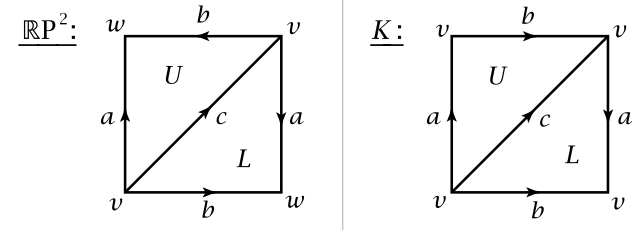
\includegraphics[width=0.6\textwidth]{Figures/Delta-RP2-Klein.png}
     \caption{}
     \label{fig:Figures/Delta-RP2-Klein.png}
 \end{figure}

 In this case, the $\Delta$-chain complex for
 $\mathbb{R}\mathbb{P}^2$ becomes

 \[
 0 \to \mathbb{Z}^2 
 \stackrel{
 \begin{pmatrix} 
     -1 & 1 \\
     1 & -1 \\
     1 & 1
\end{pmatrix} }{\to}  \mathbb{Z}^3 
\stackrel{
\begin{pmatrix} 
    1 & 1 & 0 \\
    -1 & -1 & 0
\end{pmatrix} }{\to} \mathbb{Z}^2 \to  0
 \] 
 The dual complex becomes

 \[
 0 \leftarrow \mathbb{Z}^2 
 \stackrel{
 \begin{pmatrix} 
     -1 & 1 & 1\\
     1 & -1  & 1
\end{pmatrix} }{\leftarrow}  \mathbb{Z}^3 
\stackrel{
\begin{pmatrix} 
    1 & -1\\
    1 & -1 \\
    0 & 0
\end{pmatrix} }{\leftarrow} \mathbb{Z}^2 \leftarrow  0
 \] 

 We thus find that
 $H^{2}(\mathbb{R}\mathbb{P}^2 ; \mathbb{Z}) = 0$,
 $H^{1}\left( \mathbb{R}\mathbb{P}^2;\mathbb{Z} \right) \cong
 \left<
 \begin{pmatrix} 1 \\ 1 \\ 0 \end{pmatrix} \right>
 / \left< 
 \begin{pmatrix} 1 \\ 1 \\ 0 \end{pmatrix} \right>
 \cong \mathbb{Z}$, and
 $H^{0}\left( \mathbb{R}\mathbb{P}^2; \mathbb{Z} \right) 
 \cong 
 \left< 
 \begin{pmatrix} 1 \\ -1 \\ 0 \end{pmatrix} \right>
 \cong \mathbb{Z}$.
 \end{solution}

\section{A Homotopy Construction of Cohomology}

     \begin{theorem}[]\label{Thm:SIOAJN}
         There are natural bijections
         $T \colon \left[ X, K(G,n) \right]_* \to 
         H^{n}(X;G)$ for all CW complexes $X$ and all
         $n > 0$, with $G$ any abelian group.
         Such a $T$ has the form 
         $T \left( \left[ f \right]  \right) 
         = f^{*}\left( \alpha \right) $ for a certain
         distinguished class
         $\alpha \in H^{n}\left( 
         K(G,n);G\right) $.
     \end{theorem}

     \begin{definition}[Fundamental Class]
          A class $\alpha \in H^{n}\left( 
          K(G,n);G\right) $ with the property
          stated in Theorem \ref{Thm:SIOAJN}
          is called a \textit{fundamental class}.
     \end{definition}

     \begin{note}
         The theorem also holds with
         $\left[ X,K(G,n) \right]_*$ replaced by
         $\left[ X, K(G,n) \right] $, the non-basepointed
         homotopy classes. 

         When $n>1$, every map $X \to K(G,n)$ can be
         homotoped to take basepoint to basepoint and
         every homotopy between basepoint-preserving maps can be
         homotoped to be basepoint-preserving since 
         $K(G,n)$ is simply-connected. 

         When $n=1$, 
         $\left[ X,K(G,n) \right]_* =
         \left[ X,K(G,n) \right] $ for abelian $G$ according
         to an exercise for section
         4.A in Hatcher.
         
         For  $n=0$, 
         $H^{0}(X;G) = 
         \left[ X,K(G,0) \right] $ and
         $\tilde{H}^{0}(X;G)
         = \left[ X,K(G,0) \right]_*$.
     \end{note}

     The main two steps in the proof, will be the
     following two assertions:
     \begin{enumerate}
         \item The functors
             $h^{n}(X) = 
             \left[ X,K(G,n) \right]_*$ define a
             reduced cohomology theory on the
             category of based CW complexes.
         \item If a reduced cohomology theory 
             $h^{*}$ defined on CW complexes has
             coefficient group $h^{n}(S^{0})$ which
             are zero for $n\neq 0$, then there
             are natural isomorphisms
             $h^{n}(X) \cong
             \tilde{H}^{n}(X;h^{0}(S^{0}))$ for all
             CW complexes $X$ and all $n$.
     \end{enumerate}

     Towards proving $(1)$, we will study a more
     general question: When does a sequence
     of spaces $K_n$ define a cohomology theory
     by setting $h^{n}(X) = 
     \left[ X,K_n \right]_*$? Note that
     since $\left[ X,K_n \right]_*$ is trivial when
     $X$ is a point, this will be a reduced cohomology theory.\\
     \linebreak
     
     The first part to address is putting a group
     structure on the set $\left[ X,K \right]_*$.
     When $X = S^{n}$, we have $
     \left[ S^{n},K \right]_* = 
     \pi_n (K)$, which has a group structure when
     $n>0$. The definition of this 













     \subsection{Fibrations}

     By convention, a fibration will be a map
     $p \colon E \to B$ having the homotopy lifting
     property with respect to all spaces.
     I.e., fibrations will mean Hurewicz fibrations.

     \begin{proposition}[]
         For a fibration $p \colon E \to B$, the
         fibers $F_b = p^{-1}(b)$ over
         each path component of $B$ are all
         homotopy equivalent.
     \end{proposition}

     \begin{proof}
         From a path $\gamma \colon I \to B$, we can
         construct a homotopy
         $g \colon F_{\gamma(0)} \times I \to B$ by
         $g(x,t) = \gamma(t)$. The
         inclusion $F_{\gamma(0)} \hookrightarrow E$ 
         provides a lift
         $\tilde{g}_0 \colon F_{\gamma(0)} \times \left\{ 0 \right\} 
         \to E$, so we have the following diagram:
         \begin{equation*}
         \begin{tikzcd}
             F_{\gamma(0)} \times \left\{ 0 \right\} 
             \ar[r, "\tilde{g}_0"] \ar[d, hookrightarrow] &
             E \ar[d, "p"] \\
             F_{\gamma(0)} \times I \ar[r, "g"] 
             \ar[ru, dashed, "\tilde{g}"] & B
         \end{tikzcd}
         \end{equation*}
         so since $p$ is a fibration, there exists
         a lift
         $\tilde{g} \colon
         F_{\gamma(0)}\times I \to E$ making the diagram commute.
         Hence
         $p \circ \tilde{g} = g$ maps
         $F_{\gamma(0)}$ to $\gamma(t)$ for all
         $t$, hence
         $\tilde{g}
         \left( F_{\gamma(0)} \times \left\{ t \right\} 
         \right) \subset F_{\gamma(t)}$ for all
         $t \in I$.
         In particular,
         let $L_{\gamma}$ be the
         composition
         $F_{\gamma(0)}
         \hookrightarrow F_{\gamma(0)} \times 
         \left\{ 1 \right\} \stackrel{\tilde{g}}{\to} 
         F_{\gamma(1)}$.
         The association $\gamma \mapsto L_{\gamma}$ has the
         following basic properties:

         \begin{enumerate}
             \item If  $\gamma \simeq \gamma'
                 \rel \partial I$, then
                 $L_{\gamma} \simeq L_{\gamma'}$.
                 In particular, the homotopy class
                 of $L_{\gamma}$ is independent of the choice
                 of the lifting $\tilde{g}_{t}$ of $g_t$.
             \item For a composition of paths
                 $\gamma \gamma'$, $L_{\gamma \gamma'}$ 
                 is homotopic to the composition
                 $L_{\gamma'} L_{\gamma}$.
         \end{enumerate}

         \begin{note}
             From these statement, it follows that
             $L_{\gamma}$ is a homotopy equivalence
             with homotopy inverse $L_{\overline{\gamma}}$.\\
             Note also that it is true in general that
             a fibration has the homotopy lifting 
             property for pairs $\left( X \times I,
             X \times \partial I\right) $. This is
             because 
             $\left( I \times I, I \times \left\{ 0 \right\} 
             \cup  \partial I \times I \right) 
             \cong \left( I \times I,
             I \times \left\{ 0 \right\} \right)  $ which
             naturally has the property
             that any map on
             $I \times \left\{ 0 \right\} $ can
             be extended to $I \times I$, and hence 
             $X \times \left( I \times I,
             I \times \left\{ 0 \right\} \cup 
         \partial I \times I \right) =
         \left( X \times I \times I,
         X \times I \times \left\{ 0 \right\} \cup 
     X \times \partial I \times I \right) $ also has this
     same property which is equivalent to the pair
     $\left( X \times I, X \times \partial I \right) $ having
     the homotopy extension property.
         \end{note}

         Now, to prove (a), let
         $\gamma \colon I \times I \to 
         B$ be a homotopy from
         $\gamma$ to $\gamma'$. This determines
         a family
         $g \colon F_{\gamma(0)} \times I \times I
         \to B$ with $g\left( s,t, F_{\gamma(0)} \right) 
         = \gamma(s,t)$. 
         Now we want to define a map
         $G \colon F_{\gamma(0)}\times I \times I \to 
         E$. We start by
         letting
         $G|_{F_{\gamma(0)} \times \left\{ 0 \right\} 
         \times \left\{ t \right\} }$ be
         equal to the composition
         $F_{\gamma(0)}\hookrightarrow 
         F_{\gamma(0)}\times \left\{ 1 \right\} 
         \stackrel{\tilde{g}}{\to} F_{\gamma(1)}$, and
         similarly
         $G|_{F_{\gamma(0)}\times \left\{ 1 \right\} 
         \times \left\{ t \right\} }$ but with $\gamma'$.
         Denote 
         $G|_{F_{\gamma(0)} \times 
         \left\{ s \right\} \times \left\{ t \right\} }$ 
         by $G_{s,t}$. Then
         $G_{0,t} = L_{\gamma}$ and
         $G_{1,t} = L_{\gamma'}$.
         Let
         $G|_{F_{\gamma(0)}\times 
         \left\{ s \right\} \times \left\{ 0 \right\} }$ 
         be given by the inclusion
         $F_{\gamma(0)} \hookrightarrow E$ for all
         $s$. Then using the homotopy
         lifting property for the pair
         $\left( F_{\gamma(0) } \times I,
         F_{\gamma(0)} \times \partial I\right) $, we
         can extend $G$ to a map
         $F_{\gamma(0)} \times I \times I \to B$.
         Letting now $t = 1$, we
         get a homotopy
         $F_{\gamma(0)} \times I \to B$ 
         from
         $G_{F_{\gamma(0)} \times \left\{ 0 \right\} 
         \times \left\{ 1 \right\} }
         = G_{0,1} = L_{\gamma}$ to
         $G_{1,1} = L_{\gamma'}$.\\
         For (b), if
         $\tilde{g}_t$ and
         $\tilde{g}_t'$ define $L_{\gamma}$ and
         $L_{\gamma'}$, respectively, then
         we obtain a lift defining
         $L_{\gamma \gamma'}$ by taking
         $\tilde{g}_{2t}$ for 
         $0 \le t \le \frac{1}{2}$ and
         $\tilde{g}_{2t-1}' L_{\gamma}$ for
         $\frac{1}{2} \le t \le 1$.








     \end{proof}

     \begin{definition}[Fiber-preserving]
         Given fibrations
         $p_i \colon E_i \to B$, $i=1,2$, a map
         $f \colon E_1 \to E_2$ is called 
         \textit{fiber-preserving} if
         $p_1 = p_2 f$.
     \end{definition}

     \begin{definition}[Fiber homotopy equivalence]
         A fiber-preserving map
         $f \colon E_1 \to E_2$ is a
         \textit{fiber homotopy equivalence} if there
         is a fiber-preserving map
         $g \colon E_2 \to E_1$ such that both
         compositions $fg$ and $gf$ are homotopic to the identity
         through fiber-preserving maps.
     \end{definition}

     \begin{proposition}[]
         Given a fibration
         $p \colon E \to B$ and a homotopy 
         $f_t \colon A \to B$, the pullback fibrations
         $f_0^{*}(E) \to A$ and
         $f_1^{*}\left( E \right) \to A$ are
         fiber homotopy equivalent.
     \end{proposition}

     \begin{remark}[]
         This is meant in the sense that
         there exists a fiber homotopy equivalence
         $f_0^{*}(E) \to f_1^{*}(E)$ with respect to
         these fibrations.
     \end{remark}

     \begin{corollary}
         A fibration $E \to B$ over a contractible
         base $B$ is fiber homotopy equivalent to
         a product fibration $B \times F \to B$.
     \end{corollary}

\subsubsection{Pathspace Constructions}

     \begin{definition}[Construction of]
         Given a map $f \colon A \to B$, let
         \[
         E_f := 
         \left\{ \left( a, \gamma \right)  \mid 
         a \in A, \gamma \colon 
     \left( I, \left\{ 0 \right\}  \right) \to 
 \left( B, f(a) \right) \right\} .
         \] 
         We topologize $E_f$ as a subspace of
         $A \times B^{I}$ where
         $B^{I}$ has the compact-open topology.
     \end{definition}

     \begin{proposition}[]
         The map
         $p \colon E_f \to B$ with
         $p \left( a, \gamma \right) = \gamma(1)$ is
         a fibration.
     \end{proposition}

     \begin{note}
         We have a natural embedding of $A$ as
         the set of pairs
         $(a,\gamma) \in E_f$ with
         $\gamma$ being the constant path
         at $f(a)$. Then
         $E_f$ deformation retracts onto this
         subspace by restricting all the paths
         $\gamma$ to shorter and shorter initial segments.
         The map $p \colon E_f \to B$ restricts
         to $f$ on the subspace $A$, so we have factored
         a map $f \colon A \to B$ as the composition
         $A \hookrightarrow E_f \to B$ of
         a homotopy equivalence and a fibration.
     \end{note}

     \begin{definition}[Homotopy fiber]
         The fiber $F_f$ of $E_f \to B$ is called
         the \textit{homotopy fiber} of $f$.
         It consists of all pairs
         $(a,\gamma)$ with $a \in A$ and
         $\gamma $ a path in $B$ from $f(a)$ to
         a basepoint $b_0 \in B$.
     \end{definition}

     \begin{remark}[]
         If $f \colon A \to B$ is the inclusion of a
         subspace, then $E_f$ is the space of paths
         in $B$ starting at points of $A$.
         In this case, a map
         $f \colon \left( I^{i+1},
         \partial I^{i+1}, J^{i} \right) \to 
         \left( B,A,x_0 \right) $ can be regarded
         as a map $\left( I^{i}, \partial I^{i} \right) 
         \to \left( F_f, \gamma_0 \right) $ where
         $\gamma_0$ is the constant path at $x_0$ and
         $F_f$ is the fiber of $E_f$ over $x_0$.

         Therefore, $\pi_{i+1}(B,A,x_0)$ can be identified
         with $\pi_i (F_f, \gamma_0)$, so the LES
         of homotopy groups of the pairs $(B,A)$ and of
         the fibration $E_f \to B$ can be identified (since
         also $E_f \simeq A$ ).
     \end{remark}

     \begin{definition}[]
         An important special case of the above construction is
         when $f$ is the inclusion of the
         basepoint
         $\left\{ b_0 \right\} \hookrightarrow B$.
         Then $E_f$ is the space $PB$ of paths in $B$ starting
         at $b_0$, and $p \colon PB \to B$ sends each path
         to its endpoint. The fiber
         $p^{-1}(b_0)$ is the loopspace
         $\Omega B$ consisting of all loops
         in $B$ based at $b_0$.

         Since $PB$ is contractible by progressively truncating
         paths, the LES of homotopy groups for the
         path fibration $PB \to B$ yields another
         proof that
         $\pi_n (X,x_0) \cong \pi_{n-1}\left( \Omega
         X, x_0\right) $ for all $n$.
     \end{definition}

     \begin{theorem}[Milnor 1959, \cite{Hatcher}]
         The loopspace of a CW complex is homotopy equivalent
         to a CW complex.
     \end{theorem}





     \begin{proposition}[]
         If $p \colon E \to B$ is a fibration, then
         the inclusion $E \hookrightarrow E_p$ is a fiber
         homotopy equivalence. In particular, the
         homotopy fibers of $p$ are homotopy equivalent to
         the actual fibers.
     \end{proposition}

     \begin{proof}
         Using that $p$ is a fibration, we apply
         the HLP to the homotopy
         $g \colon E_p \times I \to B$ given by
         $g\left( \left( e, \gamma \right) ,t \right) 
         = \gamma(t)$, with the initial lift
         $\tilde{g}_0 \colon E_p \times \left\{ 0 \right\} 
         \to E$ given by
         $\tilde{g}_0 \left( (e,\gamma),0 \right) = 
         e$.
         This is indeed a lift
         on $E_p \times \left\{ 0 \right\} $ since
         $g ((e, \gamma),0) =
          \gamma(0) = p(e) = p \circ
          \tilde{g}_0 \left( \left( e, \gamma \right) ,0
          \right) $.
          Given the homotopy $\tilde{g} \colon E_p \times I \to E$,
          we can now construct a homotopy
          $h \colon E_p \times I \to E_p$ by
          $h\left( (e, \gamma), t \right) 
          = \left( \tilde{g}\left( (e, \gamma), t \right) ,
          \gamma \circ \varphi_{\left[ t,1 \right] } \right) $, where
          $\varphi_{\left[ t,1 \right] } \colon
          \left[ 0,1 \right] \to \left[ t,1 \right] $ reparametrizes
          $\left[ 0,1 \right] $ to $\left[ t,1 \right] $.
          Since $p \circ \tilde{g} = g$, we have
          that
          $p \circ \tilde{g}\left( (e,\gamma), t \right) 
          = g\left( (e,\gamma),t \right) 
          = \gamma(t) = \gamma \circ \varphi_{\left[ t,1 \right] }
          (0)$, so $h$ is indeed a map
          $E_p \times I \to E_p$.
          Also, since the endpoints of the
          $\gamma$ are unchaged, $h|_{E_p \times \left\{ t \right\} 
          }$ is fiber-preserving:
          $ p \left( e, \gamma \right) = \gamma(1)
          = \gamma \circ \varphi_{\left[ t,1 \right] }(1)
          = p \circ 
          h|_{E_p \times \left\{ t \right\} }
          \left( e, \gamma \right) $.

          Next note that
          $h_0 \left( e,\gamma \right) 
          = \left( \tilde{g}\left( (e,\gamma),0 \right) ,
          \gamma \right) =
          \left( e, \gamma \right) $, so
          $h_0 = \id$. Also,
          $h_1 \left( e,\gamma \right) 
          = \left( \tilde{g}\left( (e,\gamma), 1 \right),
          \gamma(1) \right)$ which belongs to the elements
          of $E_p$ for which the path is constant - this is
          precisely what we identified $E$ with, so
          $h_1 (E_p) \subset E$. Also
          $h \left( (e, c_{p(e)}),t \right) 
          = \left( \tilde{g}\left( (e,c_{p(e)}),t \right) ,
          c_{p(e)} \circ \varphi_{\left[ t,1 \right] } \right) $ 
          which likewise belongs to $E$, so
          $h\left( E \times I \right) \subset E$.
          Let $i$ denote the inclusion
          $E \hookrightarrow E_p$. Then
          $i \circ h_1 \simeq \id$ via
          $h$ and $h_1 i \simeq \id$ via
          $h$, so $i$ is a fiber
          homotopy equivalence.

          Now, recall that
          a map $f \colon E_1 \to E_2$ is fiber preserving
          if $p_1 = p_2 f$, or, in other words,
          if $f \left( p_1^{-1}(b) \right) \subset 
          p_2^{-1}(b)$. 
          Let $q \colon E_p \to B$ be one fibration
          and $p \colon E \to B$ the other.
          Then let $F_{p,b}$ be the fiber
          above $b$ for $p$ and
          $F_{q,b}$ the fiber above $b$ for $q$.

          Since then
          since $i$ and $h_1$ are fiber-preserving, they
          restrict to maps
          $F_{p,b} \to F_{q,b}$ and
          $F_{q,b} \to F_{p,q}$, respectively,
          whose compositions are homotopic to the identity,
          so $F_{p,q} \simeq F_{q,b}$ for each
          $b \in B$, showing that
      the fibers and homotopy fibers of $p$ are homotopy
  equivalent.
\end{proof}


     We have seen that loopspaces occur as fibers
     of fibrations $PB \to B$ with contractible
     total space $PB$. Here is something of a converse:

     \begin{proposition}[]
         If $F \to E \to B$ is a fibration or fiber
         bundle with $E$ contractible, then
         there is a weak homotopy equivalence
         $F \to \Omega B$.
     \end{proposition}

     \begin{proof}
         Composing a contraction of $E$ with a projection
         $p \colon E \to B$, we obtain for each
         point $x \in E$ a path
         $\gamma_x$ in $B$ from $p(x)$ to a basepoint
         $b_0 = p(x_0)$, where $x_0$ is the point to which
         $E$ contracts.
         This yields a map $E \to PB, x\mapsto \overline{\gamma_x}$ 
         whose composition with the fibration
         $PB \to B$ sending
         sending a path in $B$ starting at $b_0$ to
         its endpoint, is $p$.
         By restriction, this then gives
         a map $F \to \Omega B$, where
         $F = p^{-1}(b_0)$, and the LES of
         homotopy groups for $F \to E \to B$ maps
         to the LES for 
         $\Omega B \to PB \to B$ (by section 6.6 in the 
         AlgTop1 notes)
         Since $E$ and $PB$ are contractible, the five-lemma
         implies that $F \to \Omega B$ is a weak homotopy
         equivalence.
     \end{proof}

     \subsubsection{Puppe Sequence/Fibration Sequence}

     Given a fibration $p \colon E \to B$ with
     fiber $F = p^{-1}(b_0)$, we know that the
     inclusion of $F$ into the homotopy fiber
     $F_p$ is a homotopy equivalence. Recall
     that $F_p $ consists of pairs
     $(e, \gamma)$ with $e \in E$ and
     $\gamma$ a path in $B$ from $p(e)$ to $b_0$.
     The inclusion $F \hookrightarrow E$ extends
     to a map $i \colon F_p \to E,
     i(e, \gamma) = e$ which is obviously a fibration.
     In fact, it is the pullback via $p$ of the path
     fibration $PB \to B$ which sends each
     path to its endpoint.

     This allows us to iterate, taking
     the homotopy fiber $F_i$ with its map to
     $F_p$, and so on, as in the first row of the
     following diagram:
     \begin{equation*}
     \begin{tikzcd}
         \ldots \ar[r] & F_j \ar[r] \ar[d, "\simeq"] &
         F_i \ar[r, "j"] \ar[d, "\simeq"] &
         F_p \ar[r, "i"] \ar[d, "\simeq"] & E \ar[r, "p"] 
         \ar[d, equal] &
B \ar[d, equal] \\
             \ldots \ar[r] & \Omega E \ar[r, "\Omega p"] &
         \Omega B \ar[r] & F \ar[r] & E \ar[r, "p"] & B
     \end{tikzcd}
     \end{equation*}








     \section{Cohomology in terms of geometry}

     \subsection{Terminology}


     Recall the following definitions:

     \begin{definition}[$k$-forms]
         Let
         \[
         L^{k}(V) := 
         \left\{ \text{multilinear forms }
         \underbrace{V \times \ldots \times V}_{k \text{ times}}
     \to F \right\} 
         \] 
         which equals $\Bil (V)$ when $k = 2$.
         The elements of $L^{k}(V)$ are called
         \textit{$k$-forms}.
     \end{definition}

     \begin{definition}[Alternating $k$-forms]
         A $k$-form $w \in L^{k}(V)$ is called
         \textit{alternating} if $w\left( v_1,\ldots,
         v_k\right) = 0$ for every $k$-tuple of vectors
         with two vectors equal.
         The vector space of alternating $k$-forms
         is denoted
         $A^{k}(V)$.
     \end{definition}

     \begin{definition}[]
         We define an action
         of $S_k$ on $L^{k}(V)$ as follows.
         For $\sigma \in S_k$ and $w \in L^{k}(V)$, define
         $\sigma \cdot w \in L^{k}(V)$ by
         \[
         \sigma \cdot w\left( v_1, \ldots, v_k \right) 
         = 
         w \left( v_{\sigma (1)},\ldots,
         v_{\sigma (k)}\right) .
         \] 
     \end{definition}

     \begin{definition}[Skew forms]
         $w \in L^{k}(V)$ is called
         \textit{skew} if $\sigma \cdot w = 
         \sgn (\sigma) w$ for all
         $\sigma \in S_k$.
     \end{definition}

     \begin{lemma}[]
         Every alternating $k$-form is skew, and
         if $\Char F \neq 2$, then every skew
         $k$-form is alternating.
     \end{lemma}

     \begin{definition}[]
         The determinant $\det (A)$ of $A$ is
         the scalar that satisfies
         \[
         w \left( A v_1, \ldots, Av_n \right) 
         = \det \left( A \right) 
         w \left( v_1, \ldots, v_n \right) 
         \] 
         for all $w \in A^{n}(V)$ and all $v_1,\ldots, v_n$.
     \end{definition}

     \begin{definition}[]
         Let $I \subset \left\{ 1,\ldots, n \right\} $ with
         elements $1 \le i_1 < \ldots < i_k \le n$.
         We define $k$-forms $y_I = 
         y_{i_1} \cdots y_{i_k}$ and
         $\widehat{y_I} = 
         \Sigma_{\sigma \in S_k} \sgn (\sigma)
         \sigma \cdot y_I$ in $L^{k}(V)$.
     \end{definition}

     \begin{theorem}[]
         Let $0 \le k \le n$. The dimension
         of $A^{k}(V)$ is 
         $\begin{pmatrix} n\\k \end{pmatrix} $ and the
         set of all $\widehat{y_I}$, where
         $I \subset \left\{ 1, \ldots, n \right\} $ has
         $k$ elements, is a basis.
     \end{theorem}

     \subsection{Wedge product/exterior product}

     Let us define first a bilinear map
      $A^{k}(V) \times A^{l}(V) \to A^{k+l}(V)$
      for all integers $k,l\ge 0$.
      Let $m = k+l$.

      Consider the product $S_k \times S_l$ as a
      subgroup of $S_m$ by letting
      $\left( \sigma, \tau \right) \in 
      S_k \times S_l$ act
      on $\left\{ 1, \ldots, m \right\} $ through the
      permutation $\pi$ given by
      \[
      \pi(i) = \sigma(i), \,
      \pi(k+j) = k + \tau(j), \quad
      1 \le i \le k, 1 \le j \le l,
      \] 
      which leaves invariant the two sets
      $\left\{ 1,\ldots, k \right\} $ and
      $\left\{ k+1,\ldots,m \right\} $.
      Denote by $\left[ \pi \right] $ the coset
      in $S_m / \left( S_k \times S_l \right) $ corresponding
      to a permutation $\pi \in S_m$.

      \begin{lemma}[]
          Let $w_1 \in L^{k}(V)$ and
          $w_2 \in L^{l}(V)$. Then
          \[
          V^{m} \ni \left( v_1, \ldots,
          v_m\right) \mapsto 
          w_1 \left( v_1,\ldots, v_k \right) 
          w_2 \left( v_{k+1},\ldots, v_m \right) \in F
          \] 
          defines an $m$-form $w_1 \cdot  w_2 \in 
          L^{m}(V)$. If $w_1 \in A^{k}(V)$ and
          $w_2 \in A^{l}(V)$, then
          \[
          w_1 \wedge w_2 = 
          \Sigma_{\left[ \pi \right] \in 
          S_m / \left( S_k \times S_l \right) }
          \sgn (\pi) \pi \cdot \left( w_1 \cdot w_2 \right) 
          \] 
          defines an alternating $m$-form
          $w_1 \wedge w_2 \in A^{m}(V)$.
      \end{lemma}

      \begin{definition}[Wedge product/exterior product]
          The alternating $m$-form
          $w_1 \wedge w_2$ is called the
          \textit{wedge product} of $w_1 $ and $w_2$.
          By linear extension, it gives a binary operation
          on
          \[
          A(V) := \bigoplus_{k=1}^{\infty}
          A^{k}(V) = \bigoplus_{k=1}^{n} A^{k}(V)
          \] 
          which becomes an algebra, called the
          \textit{alternating algebra} of $V$.
      \end{definition}

      The operation is associative.

      \begin{lemma}[]
          If $w \in A^{p}(V)$ and
          $\eta \in A^{q}(V)$, then
          \[
          w \wedge \eta = (-1)^{pq} \eta \wedge w.
          \] 
          So the wedge product makes
          $A(V)$ into a graded anticommutative ring.
      \end{lemma}

      \subsection{The cotagent space}

      Let $M$ be an $m$-dimensional smooth manifold, and let
      $p \in M$.

      \begin{definition}[]
          The dual space $(T_pM)^{*}$ of
          $T_p M$ is denoted $T_p^{*}M$ and called
          the \textit{cotangent space} of $M$ at $p$. Its
          elements are called cotangent vectors
          or covectors.
      \end{definition}

      \begin{example}[]
          For $f \in C^{\infty}(M)$,
          $df_p \in T_p^{*}M = 
          \Hom \left( T_p M, \mathbb{R} \right) $.

          Hence, in particular for $f$ the coordinate
          maps, we get that
          $dx_i(p) = d(x_i)_p \in 
          T_p^{*}M$ for all $p$ in the domain of the
          chart for $(x_i) $.
      \end{example}

      \begin{lemma}[]
          For $\left( U, (x^{i}) \right) $ a chart
          on $M$, let $p \in U$. Then
          the dual basis of
          $\left (\frac{\partial}{\partial x^{i}}|_p \right)$ is
          $\left( dx_i(p) \right)$.
      \end{lemma}

      \begin{proof}
          \[
          dx_i(p) \left( \frac{\partial}{\partial x^{j}}|_p \right) 
          = \frac{\partial x^{i}}{\partial x^{j}}(\widehat{p}) 
          \frac{d}{dt}|_{x_i(p)} =
          \delta_{i,j} \frac{d}{dt}|_{x_i(p)}
          \] 
          where we used that
          \[
          df_p\left( \frac{\partial}{\partial x^{i}}|_{p} \right) 
          = \frac{\partial \widehat{f}^{j}}{\partial x^{i}}
          (\widehat{p}) \frac{\partial}{\partial y^{j}}|_{f(p)}
          \tag{Lee (3.10)}
          \] 
      \end{proof}
      
      \subsection{Covector fields}

      \begin{definition}[Covector field]
          A \textit{covector field} $\xi$ on
          $M$ is an assignment of covectors
          \[
          \xi(p) \in T_p^{*}(M)
          \] 
          to each $p \in M$. It is called
          \textit{smooth} if, for each chart
          $\sigma \colon U \to M$ in a given atlas
          of $M$, there exist smooth functions
          $a_1, \ldots, a_m \in C^{\infty}(\sigma(U))$ such that
          \[
          \xi (p) = \sum_i a_i(p) dx_i(p)
          \] 
          for all $p \in \sigma(U)$. The space of
          smooth covector fields is denoted
          $\mathfrak{X}^{*}(M)$.
      \end{definition}

      \begin{note}
          Note that a covector $\xi(p)$ can be applied to
          the tangent vectors in $T_pM$, so
          if $U \subset M$ is open, for example, and
          $Y$ is a vector field on $U$, then
          we can define
          $\xi (Y) \colon U \to \mathbb{R}$ by
          \[
          \xi(Y) (p) = \xi(p) \left( Y(p) \right) .
          \] 
      \end{note}

      \begin{lemma}[]
          Let $\xi$ be a covector field on $M$. Then
          $\xi$ is smooth if and only if
          for each open set $U \subset M$ and each smooth
          vector field $Y \in \mathfrak{X}(U)$, the
          function $\xi (Y)$ belongs to $C^{\infty}(U)$.
      \end{lemma}

      \begin{proof}
          Suppose
          $\xi$ is smooth. Let $U$ be open and
          $(x^{i})$ a chart. For each
          $Y \in \mathfrak{X}(U)$, we write
          $Y(p) = \Sigma b_j(p) \frac{\partial}{\partial x^{i}}|_{p}$,
          where the $b_j(p)$ are smooth as functions
          of $p$ by assumption on $Y$ being smooth.
          Now
          \[
          \xi(Y) (p) = 
          \xi(p) \left( Y(p) \right) 
          = \Sigma_i a_i(p) dx_i(p)
          \left( \Sigma_j b_j(p) \frac{\partial}{\partial x^{i}}
          |_{p} \right) =
          \Sigma_i a_i (p) b_i(p)
          \] 
          since
          $dx_i(p) \left( \frac{\partial }{\partial x^{j}}
          |_{p}\right) = \delta_{i,j}$. Thus
          $\xi(Y)$ is smooth.\\

          Conversely, suppose $\xi(Y)$ is smooth. Let
          $Y = \frac{\partial}{\partial x^{i}}$, and
          $a_i(p) = \xi(p) \left( 
          \frac{\partial}{\partial x^{i}}|_p \right) $.

          Then $\xi(Y) =
          \xi (p) \left( Y(p) \right) 
          = \xi(p) \left( \frac{\partial}{\partial x^{i}}|_p
          \right) =
          a_i(p)$ is smooth by assumption.
          Now, since
          $\left( dx_i(p) \right) $ is the dual basis
          to $\left( \frac{\partial}{\partial x^{i}}|_p \right) $,
          we get that because
          $\xi(p) \left( \frac{\partial }{\partial x^{i}}|_p
          \right) = a_i(p)$, we can thus write
          \[
          \xi(p) = \sum_{i} a_i(p) dx_i(p).
          \] 
          Hence $\xi$ is a smooth covector field as
          $a_i$ is smooth.
      \end{proof}

      \begin{note}
          If $\xi$ is a smooth covector field on
          $M$ and $\varphi  \in C^{\infty}(M)$, then
          $\varphi \xi$ is again a smooth covector field on
          $M$ defined by
          $\left( \varphi \xi \right) (p) = 
          \varphi (p) \xi(p)$.
      \end{note}

      \begin{lemma}[]
          If $f \in C^{\infty}(M)$, then
          $df$ is a smooth covector field on $M$.
          For each chart $\sigma $ on $M$, the expression
          for $df$ by means of the coordinate basis is
          \[
          df = \sum_{i=1}^{m} \frac{\partial (f \circ
          \sigma)}{\partial u_i} dx_i \tag{A}\label{SMDOAW}
          \] 
          The differentials satisfy the rule
          $d(fg) = g df + f dg$ for all
          $f,g \in C^{\infty}(M)$.
      \end{lemma}

      \begin{proof}
          Smoothness and the rule for 
          $d(fg)$ follow from
          \eqref{SMDOAW}.
          To show \eqref{SMDOAW}, we apply 
          $df$ at an arbitrary point $p$ in
          a chart on $M$ first to
          obtain a covector and then apply this covector
          to the standard covector basis.
          So suppose $\left( U, (x^{i}) \right) $ is a 
          chart and $p \in U$.
          Then
          \[
          df_p \left( \frac{\partial}{\partial x^{i}}|_p \right) 
          = \frac{\partial \widehat{f}}{\partial x^{i}}(p)
          \frac{d}{dt}|_{\widehat{p}_i}.
          \] 
          So writing
          $df_p$ in terms of
          $dx_i(p)$, we get
          \[
          df_p = \sum_{i=1}^{m} 
          \frac{\partial \widehat{f}}{\partial x^{i}}(p)
          dx_i(p)
          \] 
      \end{proof}

      \begin{example}[]
          Let $M = \mathbb{R}^2$ with coordinates
          $(x_1, x_2)$ and $f \in C^{\infty}(\mathbb{R}^2)$.
          Then
          \[
          df = \frac{\partial f}{\partial x_1} dx_1 +
          \frac{\partial f}{\partial x_2} dx_2.
          \] 
      \end{example}

      \begin{definition}[Exact covector field]
          A smooth covector field 
          $\xi = a_1 dx_1 + a_2 x_2$ with
          $a_1,a_2 \in C^{\infty}(\mathbb{R}^2)$ is said
          to be \textit{exact} if it has the form
          $df$ for some function $f$.
      \end{definition}



      \subsection{Differential Forms}

      \begin{definition}[$k$-form]
          A $k$-form
          $w$ on $M$ is an assignment of an element
          \[
          w(p) \in A^{k}(T_pM)
          \] 
          for each $p \in M$.
      \end{definition}

      \begin{note}
          Given a chart $\left( U, (x^{i}) \right) $ on
          $M$, the elements
          $dx_{i_1} \wedge \ldots \wedge
          dx_{i_k}$ where $1 \le i_1 < \ldots <
          i_k \le m$ are $k$-forms on the open
          subset $\sigma (U)$ of $M$.
          For each $p \in U$, a basis for
          $A^{k}\left( T_pM \right) $ is obtained
          from these elements, so every
          $k$-form $w$ on $M$ has a unique expression
          on $U$ given by
          \[
          w = 
          \sum_{I = \left\{ i_1,\ldots,i_k \right\} }
          a_I dx_{i_1} \wedge \ldots \wedge dx_{i_k}
          \] 
          where $a_I \colon U \to \mathbb{R}$.
      \end{note}

      \begin{definition}[Smooth/differential $k$-form]
          We call $w$ \textit{smooth} or 
          \textit{differential} if all the
          functions $a_I$ are smooth, for each
          chart $\sigma$ in an atlas of $M$. The
          space of differential $k$-forms on $M$ is denoted
          $A^{k}(M)$.
      \end{definition}





    %\printbibliography



\end{document}
